\documentclass[a4paper, 11pt]{article}

\usepackage{amsmath}
\usepackage{amssymb}
\usepackage{titlesec}
\usepackage[utf8]{inputenc}
\usepackage[margin=1.5cm]{geometry}
\usepackage{prftree}
\usepackage{changepage}
\usepackage{enumitem}
\usepackage{minted}
\usepackage{lmodern}
\usepackage{graphicx}
\usepackage{wrapfig}
\usepackage{ulem}
\usepackage{marvosym}
\usepackage{xcolor}
\usepackage{mathtools}
\usepackage{bm}

\title{\vspace{-2cm}Information Theory\vspace{-1.5cm}}
\author{}
\date{}

\setlength{\parindent}{0cm}
\setlength{\parskip}{2mm}
\setlist{nosep}

% Make ~ look more normal
\let\oldsim\sim
\renewcommand{\sim}{{\oldsim}}

\newmintinline[monospace]{text}{escapeinside=\#\#, mathescape, fontsize=\normalsize}
\newminted[monospacefigure]{text}{frame=lines, framesep=1mm, autogobble, escapeinside=\#\#, mathescape, breaklines}

\titlespacing{\section}{0mm}{2mm}{2mm}
\titlespacing{\subsection}{0mm}{2mm}{2mm}
\titlespacing{\subsubsection}{0mm}{2mm}{2mm}

\newcommand{\triple}[3]{\{#1\}\;#2\;\{#3\}}
\newcommand{\triplem}[3]{\(\triple{#1}{#2}{#3}\)}
\newcommand{\ttriple}[3]{[#1]\;#2\;[#3]}

\newcommand{\interp}[2][]{\mathcal{#1}[\![#2]\!]}

\newcommand{\lightning}{\text{\Lightning}}

\newcommand{\doubleplus}{+\kern-1.3ex+\kern0.8ex}
\newcommand{\ditto}{\text{---}\cdot\cdot\,\text{---}}

\begin{document}
\maketitle

\begin{itemize}
\item Not expected to perform integrals: just reason about their behaviour and compare without actually performing. In particular, can pull eg.\ \(\log(f(x)^2) = 2\log(f(x))\). Limits are useful.
\item Expected to remember random formulae and their context, and vaguely why they work.
\item Remember that bandwidth is maximum frequency, capacity is related to bandwidth. Higher signal-to-noise ratio is better.
\item Fourier transforms switch from time to frequency. Multiplication in one domain is convolution in the other.
\item `Attenuates' means `goes to 0'.
\item Decibel: \(x = \bm{10}\log_{10}(y)\). \(x\) is \(y\)dB.
\end{itemize}

\section*{Probability Rules}
{
    For individual events \(A\) and \(B\):
    \begin{description}
    \setlength{\itemsep}{3mm}
    \item[Product Rule:] \(\displaystyle p(A,B) = p(A \mid B)p(B) = p(B \mid A)p(A)\), the `joint probability of both \(A\) and \(B\)'.
    \item[Bayes' Theorem:] \(\displaystyle p(B  \mid A) = \frac{p(A \mid B)p(B)}{p(A)}\).\\Bayes' Theorem is powerful as it lets us reverse conditioning on a variable, as well as swap the conditioning order (\(p(A \mid B)\) into \(p(B \mid A)\).
    \item[Sum Rule:] \(\displaystyle p(A) = \sum_B{p(A,B)} = \sum_B{p(A \mid B)p(B)}\).
    \end{description}

    An \textbf{ensemble} is a random variable \(X\) -- a \textbf{joint ensemble} \(XY\) is an ensemble with outcomes being ordered pairs from \(\Omega(X) \times \Omega(Y)\). The probability distribution over the joint ensemble \(p(x,y)\) is the \textbf{joint probability}.

    The \textbf{marginal probability distribution} is a subset of the joint probability distribution, describing the probability of an outcome of one variable without knowing the outcome of the other:
    \[p(x=a_i) = \sum_y{p(x=a_i,y)}\]

    Generalising the product rule to ensembles, conditional probability is:
    \[p(x=a_i \mid y=b_j) = \frac{p(x=a_i,y=b_j)}{p(y=b_j)}\]
}
\section*{Entropy and Information}
{
    \begin{minipage}[t]{0.6\textwidth}
    Entropy is positive, describes how uncertain something is. Information is negative, describes how much we know of something. Both have units of bits. Logarithm makes the measures additive, which is more intuitive.

    \begin{description}
    \item[Information:] \(I = \log_2p\).
    \item[Entropy:] \(H = -I\).
    \end{description}

    Alternate interpretation of entropy is the amount of information carried by an event/symbol: how much we learn about something contextual by seeing an event.

    Depending on how entropy is calculated, the unit changes: for an event, it's just bits. For a distribution, it's bits per outcome. For a Markov process, it's bits per symbol.

    An \textbf{ensemble} is a collection of outcomes from a random variable (with probabilities that sum to 1).
    \[H = -I = -\sum_i{p_i\log p_i}\]

    Eg.\ the entropy of the English alphabet is 4.0 bits, taking into account the probabilities of each letter.
    \end{minipage}
    \hspace{3mm}
    \begin{minipage}[t]{0.35\textwidth}
    \vspace{0pt}
    \centering
    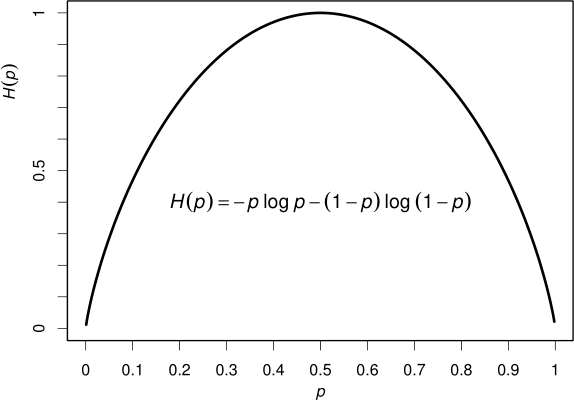
\includegraphics[width=\textwidth]{bernoulli-entropy.png}
    Entropy vs. \(p\) for a Bernoulli process (random variable with two values, of probability \(p\) and \(1-p\)).
    \end{minipage}

    \textbf{Joint entropy} is defined by:
    \[H(X,Y) = \sum_{x,y}{p(x,y)\log\frac{1}{p(x,y)}}\]

    The conditional entropy of \(X\) given that \(Y\) has taken on some specific value \(y = b_j\):
    \[H(X \mid y = b_j) = \sum_x{p(x \mid y=b_j) \log\frac{1}{p(x \mid y=b_j)}}\]

    Averaging over all possible outcomes \(Y\) might have, we get the \textbf{conditional entropy of \(X\) given \(Y\)}:
    \[H(X \mid Y) = \sum_y{ p(y) \Bigg[ \sum_x{p(x \mid y)\log\frac{1}{p(x \mid y)}} \Bigg] } = \sum_{x,y}{p(x,y)\log\frac{1}{p(x \mid y)}}\]

    \begin{minipage}[t]{0.6\textwidth}
    \textbf{Chain rule} for entropy -- relates the joint, conditional, and marginal entropies of \(X\) and \(Y\). Looks like the product rule but additive:
    \[H(X,Y) = H(X \mid Y) + H(Y) = H(Y \mid X) + H(X)\]

    \textbf{Mutual Information} between two random variables is how much information one conveys about the other:
    \[I(X;Y) = \sum_{x,y}{p(x,y)\log\frac{p(x,y)}{p(x)p(y)}}\]
    Always non-negative, \(I(X;Y) = I(Y;X)\), \(I(X;X) = H(X)\), and when \(X\) and \(Y\) are independent we have \(I(X;Y) = 0\) as expected.

    \end{minipage}
    \begin{minipage}[t]{0.35\textwidth}
    \vspace{0pt}
    \centering
    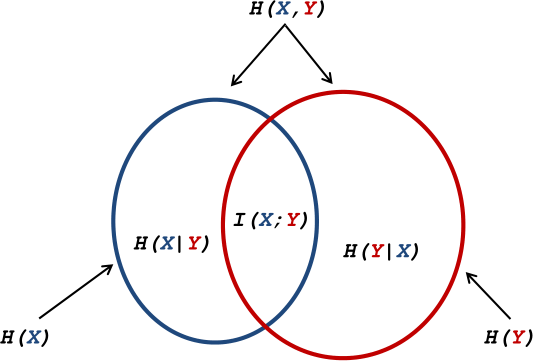
\includegraphics[width=\textwidth]{information-venn.png}
    \end{minipage}
}
\section*{Inequalities}
{
    \textbf{Independence Bound on Entropy}: as an intuitive consequence of the chain rule for entropy, we maximise the entropy of a joint distribution when the variables are independent:
    \[H(X_1,...,X_n) \leq \sum_{i=1}^n{H(X_i)}\]

    \textbf{Fano's Inequality} gives the probability of error \(P_e\) in guessing \(X\) just from knowledge of \(Y\). The lower-bound probability of error increases linearly with \(H(X \mid Y)\), how much we don't know about \(X\) given \(Y\).
    \[P_e \geq \frac{H(X \mid Y) - 1}{\log{|X|}}\]

    \textbf{The Data Processing Inequality}: if \(X\), \(Y\) and \(Z\) form a Markov chain (\(Y = f(X),Z = g(Y)\)), denoted \(X \rightarrow Y \rightarrow Z\), then mutual information is monotonically decreasing over steps along the chain. Intuitively, passing data through a pipeline can only ever decrease information.
    \[I(X;Y) \geq I(X;Z)\]
}
\section*{Distances}
{
    The \textbf{distance} \(D(X,Y)\) between \(X\) and \(Y\) is how much larger the joint entropy is than the mutual information:
    \[D(X,Y) = H(X,Y) - I(X;Y)\]

    The \textbf{Kullback-Leibler} distance or \textbf{relative entropy} between distributions \(p\) and \(q\) measures the `inefficiency' of assuming a distribution is \(p\) when it's actually \(q\). If an optimal code for \(p\) uses \(H(p(x))\) bits, then the number of \textbf{additional bits} we'd need to describe \(p\) using an optimal code for \(q\) is their distance \(D_\text{KL}(p \mid\mid q)\):
    \[D_\text{KL}(p \mid\mid q) = \sum_x{p(x)\log\frac{p(x)}{q(x)}}\]

    The requirements for a property to be a distance are that:
    \begin{itemize}
    \item \(D(X,Y) \geq 0\)
    \item \(D(X,X) = 0\)
    \item \(D(X,Y) = D(Y,X)\) (symmetry)
    \item \(D(X,Y) + D(Y,Z) \geq D(X,Z)\) (triangle inequality)
    \end{itemize}

    The \textbf{Kullback-Leibler} measure is not a distance, as it's \textbf{not symmetric}: \(D_\text{KL}(p \mid\mid q)\neq D_\text{KL}(q \mid\mid p)\).
}
\section*{Markov Processes}
{
    \begin{minipage}[t]{0.5\textwidth}
    State transition system, with probabilities as weights on each edge, labelled with an emitted symbol. The entropy of a state is the weighted sum of the probabilities of each emission (measured in bits per symbol):
    \[H = \sum_i{p_i\frac{1}{\log{p_i}}}\]

    For processes with multiple states \(s\), we can compute the entropy of the entire process by a weighted average of the entropies of each state by the probability of being in that state \(P_i\):
    \[H = \sum_s{P_s H_s}\]
    \end{minipage}
    \hspace{4mm}
    \begin{minipage}[t]{0.46\textwidth}
    \vspace{0pt}
    \centering
    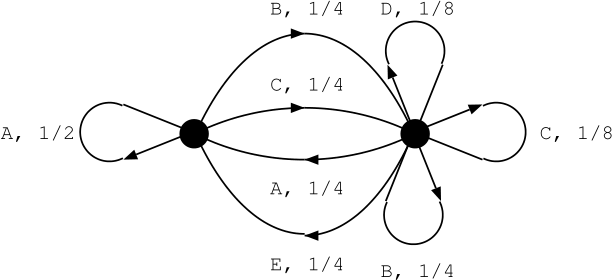
\includegraphics[width=\textwidth]{markov-process.png}
    \end{minipage}
}
\section*{Source Coding}
{
    Model sources of symbols as Markov processes: the symbols are encoded using a source encoder, and we compare the compressions and properties of the source encoders.

    The \textbf{code rate} is the \textbf{average cost of sending a symbol} in bits per symbol. Also called the \textbf{average codeword length}.

    The \textbf{efficiency} \(\eta\) of an encoding is the \textbf{information content of each bit}: the \textbf{entropy in bits per symbol divided by the code rate} (giving us the information content of each physical bit, from 0 to 1).

    \subsection*{Fixed-Length Codes}
    {
        For \(N\) symbols, use \(R = \lceil \log_2{N} \rceil\) bits and give each symbol its own value.

        In this coding the code rate is \(R\) and the efficiency \(\eta = \frac{H}{R}\).

        Fixed-length codes are inefficient:
        \begin{itemize}
        \item If \(N\) isn't a power of two, then we waste a lot of the `address space' of the fixed block size we're using.
        \item If the symbols occur with non-uniform probabilities, then \(H < \log_2{N}\) (as entropy is maximised when uniform), so we still have \(H < R\) so \(\eta < 1\).
        \end{itemize}
    }
    \subsection*{Variable-Length Codes}
    {
        \textbf{Uniquely Decodable}: A string of bits has exactly one decoding into a string of codewords. Encodings without this property normally have efficiency higher than 1.

        \textbf{Prefix Property}: No codeword is the prefix of a longer codeword. If a code satisfies this property, it's instantaneously decodable (we don't need to wait to receive more bits before starting to decode).

        \textbf{Instantaneous implies Uniquely Decodable}.

        \begin{tabular}{c | l | l | l | l}
        \(x\) & \(p(x)\) & Code 1 & Code 2 & Code 3 \\
        \hline
        A & 0.5 & 1 & 0 & 0 \\
        B & 0.25 & 00 & 10 & 01 \\
        C & 0.125 & 10 & 111 & 111 \\
        D & 0.125 & 01 & 110 & 011 \\
        \end{tabular}

        The entropy of the alphabet is 1.75 bits/symbol. 
        \begin{description}
        \item[Code 1]: Average codeword length \(R = 1.5\) bits per symbol, so efficiency \(\eta = \frac{1.75}{1.5} = 1.17\). However, it's not uniquely decodable: 1001 can be DC or ABA.
        \item[Code 2]: Average codeword length \(R = 1.75\) bits per symbol, so efficiency \(\eta = 1\) (optimal). Uniquely decodable, but doesn't satisfy the prefix property so isn't instantaneously decodable.
        \item[Code 3]: Average codeword length \(R = 1.75\) bits per symbol, so efficiency \(\eta = 1\) (optimal). Uniquely decodable and satisfies the prefix property, so is instantaneously decodable.
        \end{description}

        An alphabet of unlimited size with symbol probabilities \(\frac{1}{2^i}\) can be uniquely encoded in 2 bits per codeword by using a Huffman-style tree that's infinitely deep.
    }
    \subsection*{Shannon's Source-Coding Theorem}
    {
        A stream of data with entropy \(H\) can be compressed into a code such that the code rate/average codeword length \(R\) approaches \(H\) in the limit, but it's impossible to achieve a code rate \(R < H\) without loss of information.

        For any discrete source with entropy \(H\), and for any \(\varepsilon > 0\), it's possible to encode the symbols into a uniquely decodable code at an average rate \(R\) such that \(R = H + \varepsilon\) as \(\varepsilon \rightarrow 0\).
    }
    \subsection*{Huffman Codes}
    {
        Huffman Codes give an \textbf{optimal prefix code for any probability distribution} of symbols: intuition is to assign the most probably symbols with the shortest codewords, constructing a binary tree.

        \begin{enumerate}
        \item Start with each symbol as a singleton node, tagged with its probability.
        \item Combine the two nodes with lowest probabilities into a tree, tagging it with the sum of the probabilities.
        \item Repeat until there's only one tree.
        \end{enumerate}

        Huffman codes for the same alphabet aren't generally unique (multiple orders of choosing nodes).
    }
    \subsection*{Kraft-McMillan Inequality}
    {
        Any instantaneous code (one with the prefix property) for \(N\) codewords with lengths \(c_1 \leq c_2 \leq ... \leq c_N\) must satisfy:
        \[\sum_{i=1}^N{\frac{1}{2^{c_i}}} \leq 1\]

        This condition is \textbf{necessary but not sufficient} (use to show that a code isn't instantaneous, not that it is).

        As instantaneous implies uniquely decodable, this inequality can also disprove unique decodability.
    }
}
\section*{Channels}
{
    Consider discrete channels through which symbols pass, being corrupted in the middle.

    A \textbf{channel matrix} defines transition probabilities that if symbol \(x_i\) is injected into the channel, then \(y_j\) is emitted: \(\bm{p(y_j \mid x_i)}\).

    The probability of getting a symbol \(y_j\) is \(\displaystyle \sum_{i=1}^I{p(y_j \mid x_i)p(x_i)}\). \textbf{Remember to weight by the probability of the input symbol}, as the input distribution is usually non-uniform.

    The average probability of a symbol error \(P_e\) is the probability of getting a symbol other than the one input:
    \[P_e = 1 - \sum_{i=1}^I{p(y_i \mid x_i)p(x_i)}\]

    The \textbf{capacity of a channel} \(C\) is the \textbf{maximum} mutual information \(I(X;Y)\) between the input \(X\) and the output \(Y\) \textbf{over all possible input distributions}:

    \[C = \max_{\{p(x_i)\}}{I(X;Y)}\]

    The channel capacity is the upper bound of the code rate through the channel/the useful bits transmitted per actual bit.

    \begin{minipage}[t]{0.6\textwidth}
    For example, with the binary symmetric channel described by transition matrix:
    \[
    \begin{pmatrix}
    1 - p & p \\
    p & 1 - p
    \end{pmatrix}
    \]

    When the input distribution is \(p(x=0) = p(x=1) = 0.5\), \(H(X) = H(Y) = 1\), so \(I(X;Y) = H(X) + H(Y) + H(X,Y) = 1 + p\log p + (1-p)\log(1-p)\).

    From the plot, we can see that capacity is always maximised when the input distribution is equiprobable as above.

    Mutual information is maximised when the transition probability \(p\) is either 0 or 1 (so we deterministically know the output of the channel given the input), and the input distribution is equiprobable.
    \end{minipage}
    \begin{minipage}[t]{0.35\textwidth}
    \vspace{0pt}
    \centering
    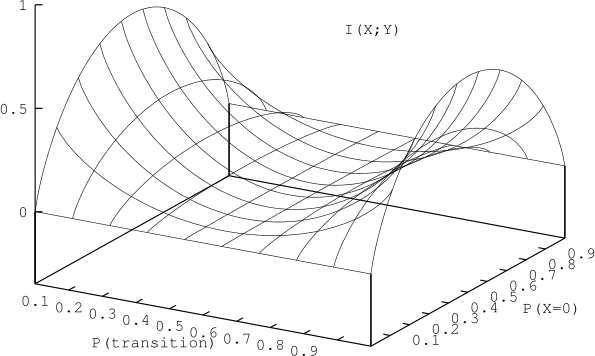
\includegraphics[width=\textwidth]{symmetric-channel.png}
    \end{minipage}
}
\section*{Error Correcting Codes}
{
    \subsection*{Repetition Codes}
    {
        Just repeat each message \(n=2m+1\) times and use majority-vote: the \textbf{code rate} is reduced by \(n\) as we're sending redundant data (so less useful information per bit), but the probability of an error getting through is:
        \[P_e = \sum_{i=m+1}^{2m+1}{\binom{2m+1}{i}p^i(1-p)^{2m+1-i}}\]
    }
    \subsection*{Channel Coding Theorem}
    {
        For a channel of capacity \(C\) and a symbol source with entropy \(H \leq C\), there exists a coding scheme such that the source is reliably transmitted through the channel with an error rate lower than an arbitrarily small \(\varepsilon\).
    }
    \subsection*{7/4 Hamming Code}
    {
        Assume we're dealing with a channel in which 0 or 1 bits are flipped in every block of 7 bits. Assume the input distributions are equally likely, so there are 128 input blocks with \(p(x_i) = \frac{1}{128}\) and entropy \(H = \log_2(128) = 7\).

        For any given input \(x_i\), there are 8 equiprobable output symbols (the input, or the input with exactly one bit flipped), so \(p(y_j \mid x_i) = \frac{1}{8}\). Finally, as the input is blocks of 7 bits, we need to divide our calculation by 7 to get the correct capacity per bit:
        \begin{align*}
        C &= \frac{1}{7}\max_{\{p(x_i)\}}{\Big(H(Y) - H(Y \mid X)\Big)} \\
          &= \frac{1}{7}\Big(7 - \sum_i \sum_j {p(y_j \mid x_i)p(x_i) \log\Big(\frac{1}{p(y_j \mid x_i)}\Big) }\Big) \\
          &= \frac{4}{7}
        \end{align*}

        \begin{minipage}[t]{0.8\textwidth}
        \setlength{\parskip}{8pt}
        Instead of 7-bit codewords, use 4 data bits and 3 parity bits for error correction.

        When transmitting data, we compute the values of the parity bits from the data bits as specified in the diagram (note that the parity bits go anticlockwise round while the data bits go clockwise):
        \begin{itemize}
        \item \(p_1 = d_1 \oplus d_2 \oplus d_4\)
        \item \(p_2 = d_3 \oplus d_1 \oplus d_4\)
        \item \(p_3 = d_2 \oplus d_3 \oplus d_4\)
        \end{itemize}
        \vspace{3mm}
        \end{minipage}
        \hspace{3mm}
        \begin{minipage}[t]{0.15\textwidth}
        \vspace{0pt}
        \centering
        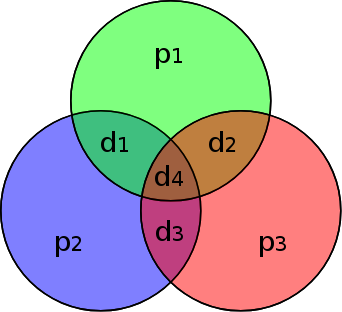
\includegraphics[width=\textwidth]{hamming74.png}
        \end{minipage}

        When receiving data, we recompute the parity bits and use them to compute \textbf{syndromes}:
        \begin{itemize}
        \item \(s_1 = p_1 \oplus d_1 \oplus d_2 \oplus d_4\)
        \item \(s_2 = p_2 \oplus d_3 \oplus d_1 \oplus d_4\)
        \item \(s_3 = p_3 \oplus d_2 \oplus d_3 \oplus d_4\)
        \end{itemize}

        To find which bit has the error, look at the diagram. If one parity bit is wrong, then that's the error. If two parity bits are wrong, then their intersection is the error. If three parity bits are wrong, then the centre's the error.

        By only carrying 4 data bits per 7 transmitted bits, the source entropy is reduced to \(H = \frac{4}{7} = C\), so the Hamming 4/7 code satisfies Shannon's Channel Coding Theorem that \(H \leq C\).

        A \textbf{perfect} error-correcting code is one which uses \(m\) bits to correct \(2^m - 1\) error patterns.
    }
}
\section*{Vector Spaces}
{
    If \(V\) is a vector space and \(v_1,...,v_n \in V\) then \(u \in V\) is a \textbf{linear combination} of \(v_1,...,v_n\).

    The \textbf{span} of a set of vectors is all linear combinations of those vectors.

    A \textbf{linear subspace} \(W\) of \(V\) is any set \(W \subset V\). Finding the representation of data in a linear subspace may amount to approximating the data or extracting just eg.\ low-frequency components. This can be called \textbf{dimensionality reduction}.

    Vectors \(v_1,...,v_n \in V\) are \textbf{linearly independent} if for scalars \(a_1,...,a_n\), we have that \(a_1v_1 + ... + a_nv_n = 0\) only if \(a_1=...=a_n=0\).

    A finite set of vectors \(v_1,...,v_n \in V\) is a \textbf{basis} for \(V\) if \(v_1,...,v_n\) are linearly independent and \(\text{span}(\{v_1,...,v_n\}) = V\), the selected vectors cover the same space as the whole set. The \textbf{dimensionality} of the space \(V\) is \(n\), the number of basis vectors.

    The \textbf{inner product} of vectors is the dot product for real and complex vectors: \(\langle -,-\rangle = \cdot\), and forms a projection of one vector onto the other. For functions \(f,g : [a,b] \rightarrow \mathbb{C}\), and where \(\overline{x}\) is the complex conjugate of \(x\), the inner product is:
    \[\langle f,g \rangle = \int_a^b{f(x)\overline{g(x)}\,dx}\]

    This is like extending the vectors to infinite length, packed as densely as the reals.

    By projecting an input vector of data \(u\) onto a vector representing a feature or pattern \(v\) (like a face), their inner product \(\langle u,v \rangle\) is a measure of how much they match up.

    Vectors are \textbf{orthogonal} if their inner product is 0, \(\langle u,v \rangle = 0\).
}
\section*{Fourier Series}
{
    Project continuous functions over the interval \([-\pi,\pi]\) into the vector space:
    \[\Bigg\{ \frac{1}{\sqrt{2}},\;\sin(x),\;\cos(x),\;\sin(2x),\;\cos(2x),\;... \Bigg\}\]

    \textbf{The Fourier Series for a function \(f\) is}:
    \begin{align*}
    & \frac{a_0}{2} + \sum_{n=1}^\infty\Big[ a_n\cos(nx) + b_n\sin(nx) \Big] \\
    a_n &= \frac{1}{\pi} \int_{-\pi}^\pi{f(x)\cos(nx)\,dx}, \qquad n=0,1,2,... \\
    b_n &= \frac{1}{\pi} \int_{-\pi}^\pi{f(x)\sin(nx)\,dx}, \qquad n=1,2,3,...
    \end{align*}

    \textbf{Need to remember in order to take the Fourier series of a function}. When manually computing a Fourier series, \textbf{find the general forms of \(a_n\) and \(b_n\) in terms of \(n\)}: then just plug them in.

    Usually very useful to know the properties of even/odd functions: rather than actually doing the integrals, can shortcut.
    \begin{itemize}
    \item If \(f,g\) are even then \(g \cdot f\) is even, same for odd, even/odd and odd/even etc.
    \item If \(f\) is odd then for \(h>0\), \(\displaystyle \int_{-h}^h{f(x)\,dx} = 0\).
    \item If \(f\) is even then for \(h>0\), \(\displaystyle \int_{-h}^h{f(x)\,dx} = 2\int_0^h{f(x)\,dx}\).
    \end{itemize}

    The Fourier series of \(f\) defines a function \(g(x)\) that is \(2\pi\) periodic: \(g(x) = g(x+2\pi)\).
}
\section*{Spectral Properties of continuous-time channels}
{
    Information-theoretic signals and channels are ultimately physical systems.

    Channels are assigned a \textbf{spectral band} of a medium, within which a \textbf{carrier signal} is modulated (by frequency, amplitude, or phase) to encode information. The resulting function has a \textbf{bandwidth} \(W\) Hz relating to the channel capacity \(C\). Bandwidth is the \textbf{range of frequencies} a signal can use.

    The original input signal is the \textbf{baseband}. The \textbf{carrier signal} is a sine wave of some frequency used as the default empty communication along the medium. The \textbf{passband} is the carrier modulated with the baseband, and is the signal that's actually transmitted. Selecting the carrier signal is `tuning' into a channel.

    \begin{minipage}[t]{0.6\textwidth}
    \setlength{\parskip}{8pt}
    \textbf{Filters} on the signal are frequency restrictions:
    \begin{itemize}
    \item Lowpass only allows small frequencies through (\(0 \leq \omega \leq x\)).
    \item Bandpass only allows a range through (\(x \leq \omega \leq y\)).
    \item Highpass only allows high frequencies through (\(x \leq \omega\)).
    \end{itemize}

    Real-values signals are symmetric about \(\omega=0\), the y-axis, so the filter is \textbf{reflected} on the negative side.
    \end{minipage}
    \hspace{3mm}
    \begin{minipage}[t]{0.35\textwidth}
    \vspace{0pt}
    \centering
    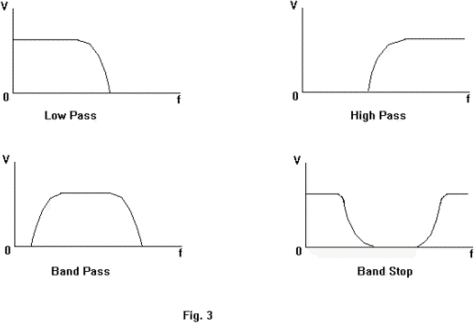
\includegraphics[width=\textwidth]{filters.png}
    \end{minipage}
}
\section*{Continuous Information}
{
    The sum rule generalises to continuous variables:
    \[p(X) = \int_{-\infty}^{\infty}{p(x,y) \, dy} \hspace{2cm} p(Y) = \int_{-\infty}^{\infty}{p(x,y) \, dx}\]

    \textbf{Differential entropy} is just normal entropy on continuous variables:
    \[H(X) = \int_{-\infty}^{\infty}{p(x) \log\frac{1}{p(x)} \, dx}\]

    Joint and conditional entropies generalise the same way:
    \[H(X,Y) = \int_{-\infty}^{\infty}\int_{-\infty}^{\infty}{p(x,y) \log\frac{1}{p(x,y)} \, dx\,dy}\]
    \[H(X \mid Y) = \int_{-\infty}^{\infty}\int_{-\infty}^{\infty}{p(x,y) \log\frac{1}{p(x \mid y)} \, dx\,dy}\]

    Mutual information also generalises:
    \[I(X;Y) = \int_{-\infty}^{\infty}\int_{-\infty}^{\infty}{p(x,y) \log\frac{p(x,y)}{p(x)p(y)} \, dx\,dy}\]
}
\section*{Noisy Channels}
{
    As with discrete variables, the capacity \(C\) of a continuous channel is the maximum mutual information over all possible input distributions \(p(x)\) for \(X\), the input.

    Entropy is maximised with equiprobable symbols: in the continuous case, \textbf{entropy is maximised by a uniform distribution}. If the signal is limited to a range/bandwidth \(v\) then \(p(x) = 1/v\) maximises entropy.

    \subsection*{Additive White Gaussian Noise (AWGN) Channels}
    {
        For any \textbf{given} variance \(\sigma^2\), the \textbf{distribution maximising entropy is Gaussian}. The mean \(\mu\) doesn't affect entropy (only spread, variance). This is important as the capacity of a channel is defined by the maximal mutual information, which depends on entropy.
        \[\bm{p(x) = \frac{1}{\sqrt{2\pi\sigma}}e^\frac{-(x-\mu)^2}{2\sigma^2}}\]

        The maximised entropy of such a distribution is (remember, can't derive):
        \[\bm{H(X) = \frac{1}{2}\textbf{log}_2(2\pi e \sigma^2)}\]

        The noise is independent of the input signal to the channel. When the \textbf{power spectral density} is \(N_0\), the \textbf{variance} \(\bm{\sigma^2 = N_0 W}\) so:
        \[H(Y \mid X) = H(N) = \frac{1}{2}\log_2(2\pi e \sigma^2) = \frac{1}{2}\log_2(2\pi e N_0 W)\]

        Then the mutual information \(I(X;Y) = H(Y) - H(Y \mid X)\) gives the \textbf{capacity} in \textbf{bits per channel `symbol'}:
        \[\bm{C = \frac{1}{2}\textbf{log}_2\Bigg(1 + \frac{P}{N_0 W}\Bigg)}\]

        Using Nyquist's theorem, we know the channel is specified completely by sampling it at \(2W\) (as the channel has lowpass bandwidth \(W\)), so we can convert the above capacity in bits per `symbol' into bits per second:
        \[\bm{C = W\textbf{log}_2\Bigg(1 + \frac{P}{N_0 W}\Bigg)}\]

        The \textbf{Signal-to-Noise ratio} SNR is \(\bm{\displaystyle \frac{P}{N_0 W}}\). Usually written in units of Decibels due to the logarithm: \(\displaystyle 10\log_{10}\Bigg(\frac{P}{N_0 W}\Bigg)\)Db.

        \textbf{Continuous-time channel capacity is primarily dictated by SNR}.
    }
    \subsection*{Noisy Channel Coding Theorem}
    {
        Summary of the above: the capacity of a continuous-time channel, lowpass bandlimited to \(W\) Hz, with additive white Gaussian noise of power spectral density \(N_0\) and bandwidth \(W\), using average transmission power \(P\), is:
        \[\bm{C = W\textbf{log}_2\Bigg(1 + \frac{P}{N_0 W}\Bigg)}\;\text{bits/sec}\]

        Increasing the bandwidth \(W\) only increases capacity up to a point: \(\displaystyle \bm{\textbf{lim}_{W \rightarrow \infty}{C} = \frac{P}{N_0}\textbf{log}_2{e}}\), whereas increasing the SNR improves the channel capacity without limit.
    }
    \subsection*{Variable Power Spectral Density}
    {
        \begin{minipage}[t]{0.6\textwidth}
        \setlength{\parskip}{8pt}
        Preceding sections assumed \(N_0\), the power spectral density, was fixed and independent of frequency (white noise). Other noise colours have different relations to frequency, usually inversely proportional or proportional at varying exponents (eg.\ pink noise has \(\displaystyle N_0 \propto \frac{1}{\omega}\))

        The information capacity of a variable-SNR channel is:
        \[\bm{C = \int_{\omega_1}^{\omega_2}{\textbf{log}_2(1 + \textbf{SNR}(\omega))\, d\omega}}\;\text{bits/sec}\]

        \(\omega_1\) and \(\omega_2\) are the upper and lower bounds of the channel bandwidth -- for a constant SNR as above this is \(W\) so the integral simplifies to just a multiplication.
        \end{minipage}
        \hspace{3mm}
        \begin{minipage}[t]{0.35\textwidth}
        \vspace{-2mm}
        \centering
        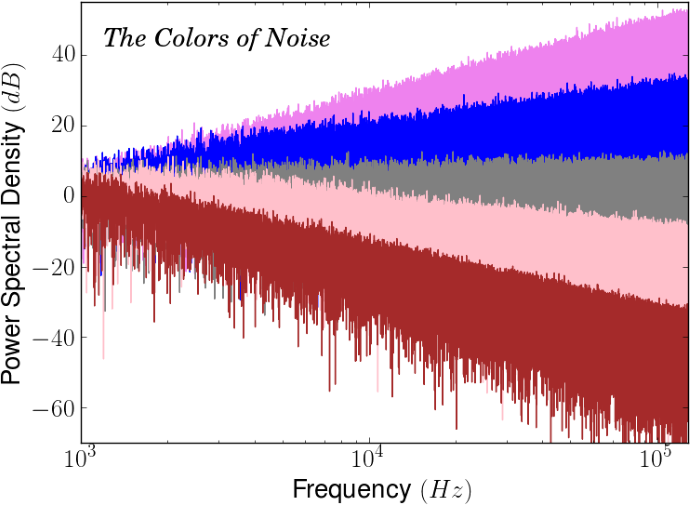
\includegraphics[width=\textwidth]{colours.png}
        \end{minipage}
    }
}
\section*{Fourier Transforms}
{
    Fourier series only work for functions periodic over \([-\pi,\pi]\). Fourier transforms work for functions with and without a period, by generalising the discrete summation into an integration. 

    Use \(F(\omega)\) or \(\mathcal{F}_f(\omega)\) to refer to the representation of \(f\) in the frequency/Fourier domain, defined by:
    \[F(\omega) = \mathcal{F}_f(\omega) = \frac{1}{2\pi}\int_{-\infty}^\infty{f(x)e^{-i\omega x}\;dx}\]

    The \textbf{inverse Fourier transform} uses \(e^{i\omega x}\) instead of \(e^{-i\omega x}\):
    \[f(x) = \int_{-\infty}^\infty{F(\omega)e^{i\omega x}\;d\omega}\]

    Compared to the Fourier series:
    \begin{itemize}
    \item We have an integration instead of a summation.
    \item Bounds now range over \([-\infty,\infty]\) rather than between the lower and upper bounds of the periodicity.
    \item The frequency parameter \(\omega\) in the exponential now ranges over \(\mathbb{R}\) instead of \(\mathbb{Z}\).
    \end{itemize}

    \begin{description}
    \item[Local-to-Global Property:] the value of \(f(x)\) at \textit{any} point \(x\) affects the value of \(F(\omega)\) at \textit{every} \(\omega\).
    \item[Global-to-Local Property:] the value of \(F(\omega)\) at \textit{any} point \(\omega\) is affected by the behaviour of \(f(x)\) at \textit{all} points \(x\).
    \end{description}

    If \(f^{(n)}(x)\) is the \(n\)\textsuperscript{th} derivative of \(f(x)\):
    \[\mathcal{F}_{f^{(n)}}(\omega) = (i\omega)^n \mathcal{F}_f(\omega)\]

    Taking the derivative of a function acts as a filtering operation in the Fourier domain: the multiplication by \((i\omega)^n\) reduces the effect of low frequencies and increases the effect of high frequencies, performing a high-pass filter.

    \textbf{Self-fourier} means that the function form stays the same: a Gaussian \(\mu, \sigma\) is self-fourier, the transformation produces \textbf{another Gaussian} \(\frac{1}{\mu},\frac{1}{\sigma}\).

    Fourier transforms can turn calculus problems into algebra problems:
    \[af''(x) + bf'(x) + cf(x) = g(x)\]
    \[\Big(a(i\omega)^2 + bi\omega + c\Big)F(\omega) = G(\omega) \hspace{1cm} F(\omega) = \frac{G(\omega)}{a(i\omega)^2 + bi\omega + c}\]
    \[f(x) = \int_{-\infty}^\infty{F(\omega) e^{i\omega x}\;d\omega}\]

    \subsection*{Convolution}
    {
        For \(f,g : \mathbb{R} \rightarrow \mathbb{C}\), the \textbf{convolution} is defined by the following. \(x\) is the relative shift.
        \[(f * g)(x) = \int_{-\infty}^\infty{f(x-y)g(y)\;dy}\]

        Convolution is commutative (\(f*g = g*f\)).

        All filtering operations are convolutions of some form, hence the importance of the operation.

        The \textbf{convolution theorem} shows that while \textbf{convolution is expensive in the time domain} (integration), it's \textbf{only a multiplication between functions in the Fourier domain}. It's usually mor efficient to transform functions into the Fourier domain, perform the multiplication, then convert back into the time domain.
        \[\mathcal{F}_{f*g}(\omega) = 2\pi \mathcal{F}_f(\omega) \mathcal{F}_g(\omega)\]

        \begin{itemize}
        \item \textbf{Convolution in the time domain is multiplication in the Fourier domain}.
        \item \textbf{Multiplication in the time domain is convolution in the Fourier domain}.
        \end{itemize}
    }
    \subsection*{Modulation}
    {
        Encoding a message (baseband) into a carrier signal to form the passband involves manipulations in the Fourier domain.

        If we want to transmit \(f(t)\), we can encode it into \(F(\omega)\) and send it directly, but that consumes the entire medium. If we modulate (multiply) \(f\) by a complex exponential \textbf{carrier signal} of frequency \(c\), \(e^{ict}\), then we \textbf{shift the Fourier spectrum up by the carrier frequency \(c\)}.
        \begin{align*}
        \mathcal{F}_{f(t)e^{ict}}(\omega) &= \frac{1}{2\pi}\int_{-\infty}^\infty{e^{ict}f(t)e^{-i\omega t}\;dt} \\
                                          &= \frac{1}{2\pi}\int_{-\infty}^\infty{f(t)e^{-i(\omega-c)t}\;dt} \\
                                          &= \mathcal{F}_f(\omega - c)
        \end{align*}

        To demodulate after receiving the signal, we just convert back to the time domain and multiply by \(e^{-ict}\).

        \textbf{Frequency modulation} alters the frequency of the wave -- rather than the height of the waves, the spacing between crests and troughs.
    }

    The \(x\)-axis is time in the time domain, frequency in the frequency domain: frequency is just 1/time.
}
\section*{Degrees of freedom in a continuous signal}
{
    Bandlimiting a function (restricting the frequency to a specific range) reduces the degrees of freedom to a finite number, allowing for quantisation.

    \subsection*{Nyquist's Sampling Theorem}
    {
        We can reconstruct a function completely as long as we sample it at least \(2W\) (twice the greatest frequency occurring in the signal). This means we sample every \(\frac{1}{2W}\) seconds.

        Define a sampling function \(\textbf{comb}(t) = \bm{\delta}_S(t) = \sum_n{\delta(t-nS)}\) as an endless sequence of tines, separated by a sampling interval \(S\). A \textbf{tine} is a Gaussian whose variance tends to 0 (the integral has area 1).

        The Fourier transform of a comb function is another comb function, but with the tines spread out as \(\frac{1}{S}\) as opposed to \(S\) in the time-domain version.

        Multiplying the time-domain function with the comb function effectively samples it at the tine locations. 

        \textbf{Convolving a function with a tine reproduces the original function centered on the tine}:
        \[\int_{-\infty}^\infty{f(t)\delta(c-t)\;dt} = f(t-c)\]
        Convolving a comb with a function produces \textbf{multiple copies of the function, each centred on a tine}.

        \begin{minipage}[t]{0.6\textwidth}
        \setlength{\parskip}{8pt}
        This means that the Fourier transform of the product of the comb function with the time-domain function produces a convolution of the frequency-domain function with the comb: as the comb is a summation of individual tines, this reproduces the Fourier transform of the function at each tine.

        Unless we sample at \(\geq 2W\), the tines in the frequency domain will be \(< 2W\) apart, which means the functions can overlap (assuming the input functions are strictly bandlimited to \(W\)). The \(2W\) defines the spacing between functions in the Fourier domain, and if they overlap then we corrupt the function being transmitted.
        \end{minipage}
        \hspace{3mm}
        \begin{minipage}[t]{0.35\textwidth}
        \vspace{0pt}
        \centering
        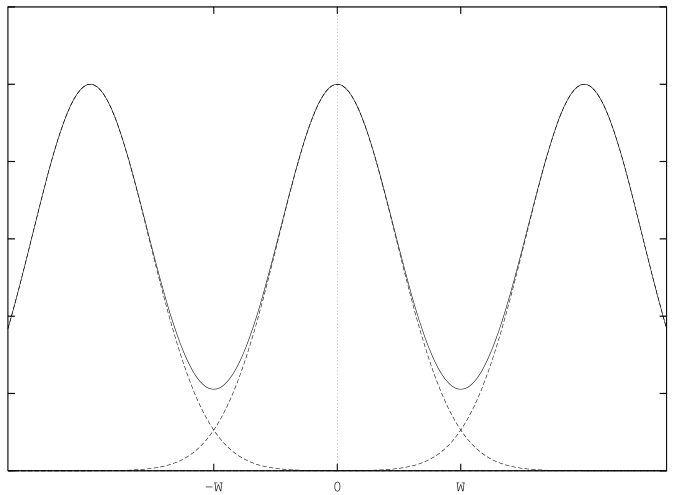
\includegraphics[width=\textwidth]{nyquist.png}
        \end{minipage}
        
        We can recover the original function by just low-pass filtering the fourier domain by \(W\), then performing an inverse Fourier transform.
    }
    \subsection*{Logan's Theorem}
    {
        For a \textbf{bandpass limited} signal where the lowest frequency is at least half the highest frequency \(W_H \leq 2W_L\), just storing the \textbf{zero-crossings} of the signal allows \textbf{reconstructing the signal with an unknown scale}.
    }
    \subsection*{Gabor's Information Diagram}
    {
        \begin{minipage}[t]{0.6\textwidth}
        \setlength{\parskip}{8pt}
        The shorter the duration of a signal, the greater its bandwidth must be: the narrower the bandwidth, the longer the signal must persist.

        \textbf{No signal can occupy an `area' smaller than \(\displaystyle \frac{1}{4\pi}\)}. The blobs are called \textbf{time-frequency atoms}.

        The unique signals with minimal areas \(\frac{1}{4\pi}\) are named \textbf{logons}, or \textbf{Gabor Wavelets}, and are \textbf{complex exponentials scaled by Gaussians}:
        \[f(x) = e^{-(\frac{x-x_0}{\alpha})^2}\;e^{i\omega_0(x-x_0)}\]

        Wavelets are helical functions of \(x\), centered on \(x_0\), frequency modulated by \(\omega_0\), and spreading constant \(\alpha\).

        Gabor wavelets have the greatest possible resolution so would be good as a basis for representing signals in, but are \textbf{non-orthogonal}, so the coefficients are hard to compute.
        \end{minipage}
        \hspace{3mm}
        \begin{minipage}[t]{0.35\textwidth}
        \vspace{0pt}
        \centering
        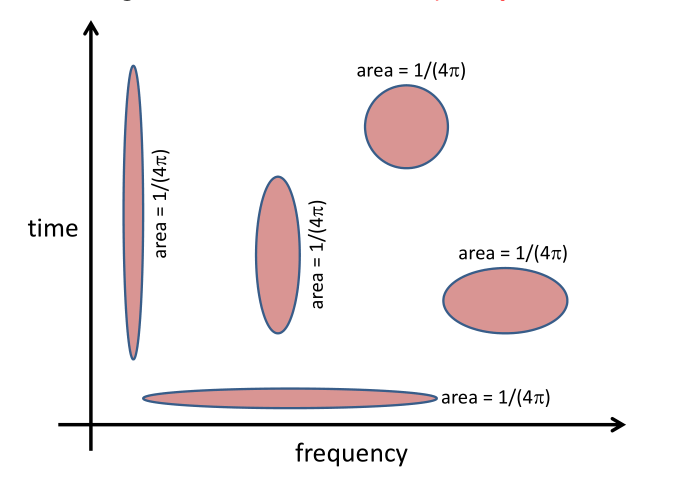
\includegraphics[width=\textwidth]{gabor-quantal.png}\\
        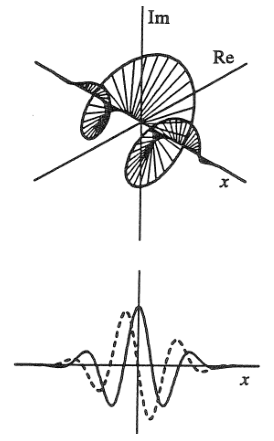
\includegraphics[width=0.5\textwidth]{gabor-wavelets.png}
        \end{minipage}
    }
}
\section*{Data Compression}
{
    Where there's redundant information, there's potential for compressibility.
    
    \begin{itemize}
    \item \textbf{RLE} removes adjacent redundancy.
    \item \textbf{Predictive coding} records deviations from a prediction rather than the larger sample values.
    \item \textbf{Dictionary compression} exploit that strings of symbols have much more varied probabilities than individual symbols, and exploit sparseness of data.
    \end{itemize}

    \textbf{LZW} and \textbf{GIF} compression works by building a \textbf{dictionary} of data: words or pixel values in one pass, then replacing each instance of the word/pixel by a reference into the dictionary. Might use variable-length indices to reduce the space needed to store a pointer to a common item.

    \textbf{Vector quantisation} is a lossy compression method that takes advantage of sparseness of language. With a coding budget of 15 bits, we can only represent strings of a few letters, and most of them are nonsense. If instead we build a \textbf{dictionary} or \textbf{codebook} of words that are used and use pointers into the table, then we represent \(2^{15}\) useful words.

    Can encode approximate values, eg.\ similar clusters of pixels can be mapped to the same code if the difference isn't noticeable.
}
\section*{FFT and DFT}
{
    Consider discrete functions instead of real/complex functions. 

    Skipping?
}
\section*{Wavelets}
{
    Wavelets are an alternative way of representing signals, combining Fourier (frequency-based) with size-specific local undulations.

    \textbf{Dyadic wavelets} are one form of wavelets, where a generating wavelet \(\Psi(x)\) spawns an orthonormal basis \(\Psi_{jk}(x)\) to represent a function \(f(x)\):
    \[f(x) = \sum_{j=-\infty}^\infty \sum_{k=-\infty}^\infty c_{jk}\Psi_{jk}(x)\]

    The \textbf{daughter wavelets} \(\Psi_{jk}(x)\) are all transformations and scales/stretches parameterised by \(j\) and \(k\) of the mother wavelet \(\Psi(x)\).

    The wavelets are local only to a specific area of the function, defined by the \(j,k\) parameters. This means that the coefficients \(c_{jk}\) carry specifically local information about the function.
}
\section*{Kolmogorov Complexity}
{
    \textbf{Algorithmic complexity} of data is the length of a program which can generate the data. Not to be confused with \textbf{computational complexity}, the cost of executing such a program.

    \textbf{Kolmogorov Complexity} measures the complexity of a string of data as the length of the shortest executable program which can compute the string, the \textbf{`minimal description length'}.

    When a data string is drawn from a distribution, \textbf{the Kolmogorov complexity is approximately equal to the entropy of the distribution}: \(H \approx K\).

    The Kolmogorov complexity of a string of bits of length \(n\) is usually around \(n\). However, some strings have significantly lower complexity, such as the binary encoding of \(\pi\): the Kolmogorov complexity for that string is constant and low, rather than infinite.

    An infinite string is \textbf{K-incompressible} if the Kolmogorov complexity \(K\) tends to the length of the string in the limit:
    \[\lim_{n\rightarrow\infty}{K(x_1x_2...x_n \mid n)} = n\]
}
\section*{Extracting Noise}
{
    Signals have precise frequencies and are periodic, whereas noise is usually random: we can extract periodic components from noise by making the noise average out against itself using an auto-correlation integral:
    \[g(t) = \int_{-\infty}^\infty{f(x)f(x + t)\;dx}\]
}
\end{document}